\documentclass[11pt,a4paper]{article}
\usepackage[margin=2.2cm]{geometry}
\usepackage{amsmath,amssymb,graphicx,booktabs,array,longtable,xcolor,enumitem}
\usepackage[hidelinks]{hyperref}
\usepackage{caption}
\captionsetup{font=small,labelfont=bf}
\newcommand{\dc}{d_c}\newcommand{\de}{d_e}
\newcommand{\ok}{\textcolor{green!50!black}{\checkmark}}
\newcommand{\bad}{\textcolor{red!70!black}{$\times$}}
\setlist{itemsep=2pt,topsep=3pt}
\emergencystretch=2em

\title{Scalable Fluid Antenna Systems for Mixed-Field Localization:\\
Reproduction Study, Parameter Audit and Improved Implementation}
\author{Technical report}
\date{\today}

\begin{document}
\maketitle

\begin{abstract}
We reimplemented the two-stage scalable fluid antenna system (S-FAS) localization algorithm
in MATLAB/Octave from two publications by the same group: the IEEE ICC 2026 conference paper
and its extended IEEE JSTSP 2026 journal version. We compare what each document states, identify
inconsistencies and errors, and reproduce the single-shot experiment (four sources at
$30\lambda$, $300\lambda$, $1000\lambda$, $5000\lambda$) under four parameter sets.
The main finding is that both papers \emph{state} element spacings $\dc=0.05\lambda$ and
$\de=0.5\lambda$, but the published figures can only be reproduced with $\dc=0.1\lambda$ and
$\de=1\lambda$. With these spacings, the algorithm exactly as published recovers all four
DOAs to within $0.05^\circ$; with the stated spacings, Stage~2 frequently fails for the Fresnel
and far-field sources. We also list about fifteen smaller errors and propose an improved
pipeline that removes a range-grid artifact present in the published setting.
\end{abstract}

\tableofcontents

%===========================================================
\section{Documents examined}
\begin{description}
\item[ICC paper] T.~Wu \emph{et al.}, ``Scalable Fluid Antenna Systems for Mixed-Field Source
Localization,'' \emph{IEEE ICC 2026}, DOI 10.1109/ICC59461.2026.11586773. Six pages; it shows only
a single-shot example (Figs.~2 and 3) and refers to the journal version (arXiv:2508.10831) as
``the transactions version''.
\item[Journal paper] T.~Wu \emph{et al.}, ``Scalable Fluid Antenna Systems: A New Paradigm for
Array Signal Processing,'' \emph{IEEE J.~Sel.~Topics Signal Process.}, vol.~20, no.~3,
pp.~389--406, Apr.~2026, DOI 10.1109/JSTSP.2026.3673981. It extends the ICC paper with error
analysis, a CRB, complexity and runtime figures, and RMSE studies (Figs.~3--11).
\end{description}
Neither paper links to code or data.

%===========================================================
\section{Method summary (common to both papers)}
An $M$-element ULA has a software-controlled spacing $d(\alpha)=\alpha d_0$, with $d_0=\lambda/2$.
Element positions are $p_m(\alpha)=(m-1)\alpha d_0$ and the aperture is $D(\alpha)=(M-1)\alpha d_0$.
The exact spatial geometry (ESG) model uses
\begin{equation}
r_{m,k}(\alpha)=\sqrt{r_k^2+p_m^2(\alpha)-2r_kp_m(\alpha)\sin\theta_k},\qquad
[\mathbf a^{\rm ESG}_k]_m=\frac{r_k}{r_{m,k}}\,e^{\,j\frac{2\pi}{\lambda}(r_{m,k}-r_k)} .
\end{equation}
\textbf{Stage 1} (compressed, $\alpha_c<1$) is modeled with the far-field manifold and a banded
Toeplitz coupling matrix $\mathbf C_c$. Keeping the central $M-2p$ elements absorbs coupling
into a diagonal source-gain matrix, after which 1-D MUSIC gives coarse DOAs $\hat\theta^{(1)}_k$.
\textbf{Stage 2} (extended, $\alpha_e$) treats coupling as negligible. For each $k$ it performs
(i) a 1-D ESG-MUSIC range search at fixed $\hat\theta^{(1)}_k$, giving $\hat r^{\rm init}_k$, then
(ii) a local 2-D ESG-MUSIC search in $|\theta-\hat\theta^{(1)}_k|\le\Delta\theta$,
$|r-\hat r^{\rm init}_k|\le\Delta r$.

%===========================================================
\section{Parameters: what each document says}
\begin{table}[!htbp]\centering\small
\caption{Simulation parameters. ``--'' means not specified. Bold entries conflict with each other.}
\label{tab:params}
\begin{tabular}{@{}p{3.6cm}p{3.1cm}p{3.4cm}p{3.9cm}@{}}
\toprule
Quantity & ICC paper & Journal (stated) & Journal (figures / text) \\
\midrule
$M$, $\lambda$ & 32, 1\,mm & 32, 1\,mm & 32, 1\,mm \\
$\alpha_c$ ($\dc$) & \textbf{0.1 ($0.05\lambda$)} & \textbf{0.1 ($0.05\lambda$)}, Sec.~II-B & \textbf{$\dc=0.1\lambda$}: Sec.~IV-A, Fig.~4, Fig.~7 legend \\
$\alpha_e$ ($\de$) & \textbf{1 ($0.5\lambda$)} & \textbf{1 ($0.5\lambda$)}, Sec.~II-B & \textbf{$\de=1\lambda$}: Sec.~IV-A, Fig.~5, CRB2 \\
SNR, $N$ (single shot) & 10\,dB, 500 & -- & -- \\
SNR, $N$ (RMSE) & -- & 0\,dB / $N{=}500$ & same \\
Monte-Carlo trials & 1000 (stated; no MC figure) & 1000 & 50 (Fig.~3 caption) \\
Stage-1 grid & -- & $0.1^\circ$ on $[-90^\circ,90^\circ]$ & same \\
1-D range grid & $[r_{\min},r_{\max}]$, -- & -- & $G_r=216$ points (runtime text) \\
$\Delta\theta$ & $5^\circ$ & $5^\circ$ & $5^\circ$ \\
$\Delta r$ & $\mathbf{0.2\,r_{\max}}$ & $\mathbf{60\lambda}$ & $60\lambda$ \\
Local grid & -- & $\delta\theta=0.015^\circ$, $\delta r=0.1\lambda$ & $667\times1201$ (consistent) \\
Coupling $\beta$ & $\approx2$ & -- & -- \\
Coupling $|c_1|$ & $\approx0.3$ (comp.), $<0.05$ (ext.) & -- & -- \\
$c_0$, $\phi_0$, $p$ & -- & -- & -- \\
Range reference & ``array center'' (text) / element 1 (eqs.) & same & same \\
\bottomrule
\end{tabular}
\end{table}

\paragraph{Assumptions in our implementation.} Neither paper gives $c_0$, $\phi_0$ or $p$. We use
$\beta=2$, choose $c_0$ so that $|c_1(\alpha_c)|=0.30$ (as in the ICC paper), and set $\phi_0=\pi/4$ and $p=1$.
Coupling is applied only in Stage~1. The true channel always uses the exact ESG model.
Independent unit-power circular Gaussian sources and independent snapshots are drawn in each
stage. MUSIC denominators are normalized by $\|\mathbf a\|^2$; without this, the $r_k/r_{m,k}$
amplitude term biases the spectrum toward small $r$.

%===========================================================
\section{Differences between the ICC paper and the journal}
\begin{longtable}{@{}p{3.6cm}p{5.6cm}p{6.4cm}@{}}
\toprule
Topic & ICC paper & Journal \\ \midrule \endhead
Scope & Method plus single-shot demo (Figs.~2--3) & Adds error analysis, CRB (Eqs.~49--50), complexity, runtime, optional coupling-robust Stage~2 (Eqs.~46--48), RMSE studies (Figs.~7--11), baseline comparison (Fig.~3) \\
Stage-1 name & ``Spatial smoothing'' & ``Central subarray selection (not to be confused with spatial smoothing)'' -- corrected \\
Far-field validity in Stage 1 & ``$r_k\gtrsim10D_c$'' & Phase-error bound $\pi D_c^2/(\lambda r_k)$; worked example at $100\lambda$ \\
Coupling matrix & Symmetric Toeplitz; $c_0$ called ``normalized self-impedance'' & Toeplitz with $c_m^*$ below the diagonal (Eq.~5); $c_0$ called ``reference coupling strength'' \\
Coupling values & $\beta\approx2$, $|c_1|\approx0.3$ / $<0.05$ & None given \\
$\Delta r$ & $0.2\,r_{\max}$ & $60\lambda$ \\
ESG justification & Asserted & Quantified: ESG vs.\ Fresnel gives 15--25\% DOA and 20--40\% range RMSE reduction \\
Field-region terms & Remark~1: near-field $r<0.62\sqrt{D^3/\lambda}$ & ``Near-field'' explicitly means radiative near-field (Fresnel region) \\
Limitations & One sentence & Stationarity condition across the switch, 2-D only, coupling overhead \\
Hardware & Cites FAS technologies & Fig.~1 prototypes, explicitly ``conceptual; no hardware measurements'' \\
\bottomrule
\end{longtable}

%===========================================================
\section{Errors and inconsistencies}
Severity: \textbf{H} affects reproducibility of results, \textbf{M} affects interpretation,
\textbf{L} is editorial.
\begin{enumerate}[label=\textbf{E\arabic*}]
\item \textbf{[H] Element spacing used in the simulations.} Both papers state $\alpha_c=0.1$, $\alpha_e=1$
($\dc=0.05\lambda$, $\de=0.5\lambda$). The journal's Sec.~II-B even says this keeps the extended spacing
``at the classical half-wavelength limit''. Yet Sec.~IV-A says ``compressing the array to $\dc=0.1\lambda$''
and ``extended configuration ($\de=1\lambda$)''; the Fig.~4 and Fig.~5 captions use the same values; the Fig.~7 legend
lists ``MUSIC ($d=0.1\lambda$)''; and the reference bound that AAR ``closely tracks'' is CRB2 for $d=1\lambda$.
Our results (Sec.~\ref{sec:repro}) confirm that the published figures require $\dc=0.1\lambda$ and $\de=1\lambda$.
\item \textbf{[H] Coupling claims inconsistent with the stated spacing.} With $\beta=2$ and $|c_1(\alpha_c)|=0.3$,
Eq.~(6) gives $|c_1(\alpha_e)|=0.3\,e^{-\beta(\alpha_e-\alpha_c)/2}$, which is $0.122$ for $(0.1,1)$ but $0.050$ for $(0.2,2)$.
Only the second matches the ICC claim ``$|c_1(\alpha_e)|<0.05$'', which independently supports E1.
\item \textbf{[H] Coupling parameters unspecified.} $c_0$, $\phi_0$ and the coupling range $p$ are never given,
and $p$ sets the subarray size $M-2p$ used in Stage~1.
\item \textbf{[H] $\Delta r$ differs between versions} ($0.2\,r_{\max}$ vs.\ $60\lambda$). Combined with the 216-point
1-D grid, $\Delta r=60\lambda$ produces a systematic $\approx5.7\%$ range bias at $1000\lambda$ (Sec.~\ref{sec:improved}).
\item \textbf{[M] Range reference point.} The text measures $r_k$ ``from the array center'', but Eqs.~(2)/(4) (ICC)
and (7)/(10) (journal) use $p_1=0$, i.e., element~1. We follow the equations.
\item \textbf{[M] ``$r_k\gtrsim10D_c$'' makes the far-field approximation valid (ICC).} The noiseless Stage-1 bias we
measure is $-1.11^\circ$ at $30\lambda$ ($\approx19D_c$) for $\alpha_c=0.1$ and $-2.2^\circ$ for $\alpha_c=0.2$
(Table~\ref{tab:bias}). The journal's bound is the more accurate statement; its $100\lambda$ example
(``$<0.5^\circ$'') agrees with our $-0.34^\circ$.
\item \textbf{[M] Inconsistent field-region labels.} With $\de=0.5\lambda$, the Fraunhofer distance is $2D_e^2/\lambda=480\lambda$;
with $\de=1\lambda$ it is $1922\lambda$. The papers call $1000\lambda$ ``far-field'' (true only for $0.5\lambda$),
while the journal quotes ``$R_F=512\lambda$'' (Sec.~IV-D), which matches neither array.
\item \textbf{[M] ICC Remark~1} defines near-field as $r<0.62\sqrt{D^3/\lambda}$ (the reactive region),
contradicting its own introduction, which uses the Fresnel region. The journal fixes this.
\item \textbf{[M] Unnormalized MUSIC.} Eqs.~(13)/(15) (ICC) and (41)/(43) (journal) use
$1/(\mathbf a^H\mathbf U_n\mathbf U_n^H\mathbf a)$ with non-unit-norm ESG vectors, which favors small $r$.
Not wrong as such, but it should be stated.
\item \textbf{[M] CRB interpretation.} CRB1/CRB2 are bounds for ideal uncoupled ULAs at $0.5\lambda$/$1\lambda$, not for the
two-stage model. The journal says so itself, but the abstract-level claims of ``near-optimal'' performance rely on CRB2,
which is only the relevant bound if $\de=1\lambda$ (E1).
\item \textbf{[L] Monte-Carlo count.} The journal text says 1000 trials; the Fig.~3 caption says 50.
\item \textbf{[L] Wrong equation references.} ICC Algorithm~1 refers to Eqs.~(14)/(15) for $\mathbf F$ and the MUSIC spectrum
(they are (9)/(11)); Algorithm~2 cites Eqs.~(16)--(19), which do not exist.
\item \textbf{[L] Leftover revision text (journal).} Sec.~III opens with ``re-formulates \ldots\ Sections III--V \ldots\ legacy
three-stage framework preserved in the previous section'', but no three-stage framework appears. The limitations
paragraph (``Despite these achievements\ldots'') sits inside Sec.~II-A, before the system design.
\item \textbf{[L] Mis-citation (journal).} ``The MUSIC algorithm [58]'' cites a Bluetooth ranging paper; Schmidt's MUSIC is [5].
\item \textbf{[L] ICC Sec.~I says the extended array uses ``super-wavelength spacing''} while specifying $\de=0.5\lambda$, which is
consistent only with $\de=1\lambda$ (supports E1).
\end{enumerate}

%===========================================================
\section{Reproduction}\label{sec:repro}
\subsection{Configurations}
All runs use the four-source scenario $\theta=[-40,-20,10,30]^\circ$, $r=[30,300,1000,5000]\lambda$, SNR $=10$\,dB,
$N=500$, $M=32$, the same random seed for the single-shot figures, and the same coupling model.
\begin{table}[!htbp]\centering\small
\caption{Configurations compared.}\label{tab:cfg}
\resizebox{\linewidth}{!}{\begin{tabular}{@{}llllll@{}}\toprule
Name & $\dc$, $\de$ & 1-D range grid & $\Delta r$ & Local grid & Stage-2 init \\ \midrule
ICC as stated & $0.05\lambda$, $0.5\lambda$ & 3000 log pts & $0.2r_{\max}=2000\lambda$ & $0.01^\circ$, 800 pts in $1/r$ & paper \\
Journal as stated & $0.05\lambda$, $0.5\lambda$ & 216 log pts & $60\lambda$ & $0.015^\circ$, $0.1\lambda$ & paper \\
Journal figure-implied & $0.1\lambda$, $1\lambda$ & 216 log pts & $60\lambda$ & $0.015^\circ$, $0.1\lambda$ & paper \\
Improved & $0.1\lambda$, $1\lambda$ & 3000 log pts & $60\lambda$ & $0.015^\circ$, $0.1\lambda$ & coarse 2-D + 2nd pass \\
\bottomrule\end{tabular}}\end{table}

\subsection{Stage 1}
\begin{figure}[!htbp]\centering
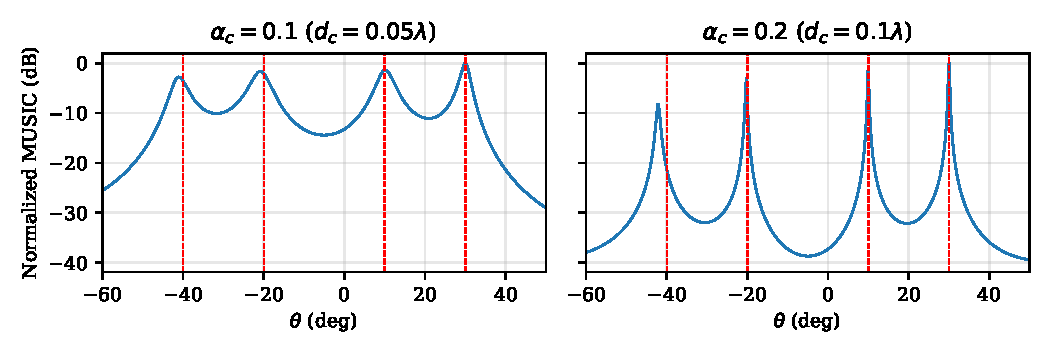
\includegraphics[width=.85\linewidth]{figs/stage1.pdf}
\caption{Stage-1 MUSIC spectra (red: true DOAs). Both spacings resolve all four sources. The $30\lambda$ source
is biased by the far-field approximation, by about $-1^\circ$ at $\dc=0.05\lambda$ and $-2^\circ$ at $\dc=0.1\lambda$.}
\label{fig:s1}\end{figure}

\begin{table}[!htbp]\centering\small
\caption{Noiseless Stage-1 bias for one source at $-40^\circ$ (no coupling, $\alpha_c=0.1$) versus range.}\label{tab:bias}
\begin{tabular}{@{}lcccccc@{}}\toprule
$r$ ($\lambda$) & 15 & 30 & 60 & 100 & 300 & 1000\\\midrule
Bias (deg) & $-2.17$ & $-1.11$ & $-0.56$ & $-0.34$ & $-0.11$ & $-0.03$\\\bottomrule
\end{tabular}\end{table}

Coupling is \emph{not} the main error source in Stage~1. With $\alpha_c=0.1$ and $p=1$, the Stage-1 DOA RMSE
(40 trials) is $0.80/0.52/0.42/0.35^\circ$ with no coupling and $0.91/0.45/0.30/0.24^\circ$ with
$|c_1|=0.3$. The limiting factors are the tiny compressed aperture ($D_c=1.55\lambda$) and the far-field bias of
the $30\lambda$ source. Increasing $\alpha_c$ improves the Fresnel and far-field sources (RMSE $0.27/0.09/0.03^\circ$ at
$\alpha_c=0.2$) but increases the near-field bias in proportion.

\subsection{Single-shot figures (equivalents of ICC Figs.~2--3 / journal Figs.~5--6)}
In each row, the solid curve is the 1-D range spectrum the algorithm actually uses (at $\hat\theta^{(1)}$); the
dotted curve is the same spectrum at the true angle; the red dashed line is the true range. In the 2-D maps,
$+$ marks the true location.

\newcommand{\cfgfig}[2]{%
\begin{figure}[!htbp]\centering
\includegraphics[width=\linewidth]{figs/fig2_#1.pdf}\\[-1mm]
\includegraphics[width=\linewidth]{figs/fig3_#1.pdf}
\caption{#2}\label{fig:#1}\end{figure}}

\cfgfig{icc}{\textbf{ICC values as stated} ($\dc=0.05\lambda$, $\de=0.5\lambda$, $\Delta r=2000\lambda$). Top: 1-D range spectra.
Bottom: local 2-D spectra. The near-field source is correct; the $300\lambda$ peak appears only because the
very wide $\Delta r$ lets the 2-D search recover from a poor $\hat r^{\rm init}$. The far-field ranges are off by 17\% and 13\%.}

\cfgfig{jstated}{\textbf{Journal grids with the stated spacing} ($0.05\lambda$/$0.5\lambda$, $\Delta r=60\lambda$). A $0.8^\circ$
Stage-1 error moves the $300\lambda$ peak to $\approx660\lambda$, and the $\pm60\lambda$ window cannot reach the true range
(final $\hat r_2=597\lambda$, $\hat\theta_2=-20.69^\circ$). The published Fig.~2(b)/Fig.~5(b) does \emph{not} look like this.}

\cfgfig{jfig}{\textbf{Journal figure-implied spacing} ($0.1\lambda$/$1\lambda$), algorithm exactly as published. The 1-D spectra
show sharp peaks at $30\lambda$, $300\lambda$ and $1000\lambda$ and a rising curve peaking near $5000\lambda$, matching the shape of the
published Fig.~2/Fig.~5. The 2-D maps go from a point-like peak to horizontal ridges, as in Fig.~3/Fig.~6.
All DOAs are within $0.05^\circ$. Source~3 shows the $\Delta r$ artifact: the true $1000\lambda$ lies just outside the window,
so $\hat r_3=1057\lambda$.}

\clearpage
\subsection{Monte-Carlo summary}
\begin{table}[!htbp]\centering\scriptsize
\caption{Monte-Carlo summary (SNR 10\,dB, $N=500$; trials with all four Stage-1 peaks resolved / total). Columns
per source: $30\lambda$, $300\lambda$, $1000\lambda$, $5000\lambda$.}\label{tab:mc}
\setlength{\tabcolsep}{2.6pt}
\begin{tabular}{@{}l|cccc|cccc|cccc|cccc@{}}\toprule
 & \multicolumn{4}{c|}{Stage-1 DOA RMSE ($^\circ$)} & \multicolumn{4}{c|}{Final DOA RMSE ($^\circ$)} &
 \multicolumn{4}{c|}{Median $|\Delta r|/r$ (\%)} & \multicolumn{4}{c}{$|\Delta r|/r<5\%$ (\% trials)}\\\midrule
ICC as stated (15/15) & 0.83 & 0.44 & 0.47 & 0.22 & 0.041 & 0.040 & 0.173 & 0.031 & 0.4 & 2.5 & 9.9 & 60.0 & 100 & 93 & 27 & 13 \\
Journal as stated (15/15) & 0.83 & 0.44 & 0.47 & 0.22 & 0.031 & 0.313 & 0.280 & 0.122 & 0.3 & 4.4 & 53.9 & 98.8 & 100 & 67 & 0 & 33 \\
Journal fig.-implied (15/15) & 2.16 & 0.30 & 0.10 & 0.04 & 0.029 & 0.008 & 0.045 & 0.028 & 0.0 & 0.2 & 5.7 & 3.4 & 100 & 100 & 0 & 87 \\
Improved (15/15) & 2.14 & 0.29 & 0.10 & 0.03 & 0.019 & 0.009 & 0.007 & 0.019 & 0.0 & 0.1 & 0.7 & 4.9 & 100 & 100 & 100 & 53 \\
\bottomrule\end{tabular}\end{table}

\noindent How to read Table~\ref{tab:mc}:
\begin{itemize}
\item \textbf{Stated spacing (rows 1--2).} The near-field source is always correct, but the $1000\lambda$ and $5000\lambda$
ranges fail in most trials. With the journal's $\Delta r=60\lambda$ (row~2), the $300\lambda$ source also fails in a third of
the trials, because the window cannot recover from a wrong $\hat r^{\rm init}$.
\item \textbf{Figure-implied spacing (row 3)} gives final DOA RMSE $\le0.05^\circ$ for all sources and $<0.3\%$ range error at
$30\lambda$ and $300\lambda$, consistent with the published claims. The $1000\lambda$ result is a constant $5.7\%$ in \emph{every}
trial: $\hat r^{\rm init}$ snaps to the 216-point grid node at $1117\lambda$, and the estimate sits at the window edge
$1057\lambda$. The $5000\lambda$ ``success'' is the same artifact in reverse: a grid node at $4931\lambda$ puts the window edge
at $4991\lambda$, close to the truth by coincidence.
\item \textbf{Improved (row 4)} removes the grid artifact: $1000\lambda$ is now within $5\%$ in all trials (median $0.7\%$), and
all final DOAs improve. The $5000\lambda$ source is beyond the Fraunhofer distance ($1922\lambda$), so its range is only weakly
identifiable; with the artifact removed, its true accuracy shows (median $4.9\%$). Rows 1--3 use one random stream
(seed 10); row~4 uses per-trial seeds after a restart (trials 1--3 from seed 10), so draws differ slightly.
\end{itemize}

%===========================================================
\section{Which values reproduce the published figures?}
The published single-shot figures are reproduced, in shape and in accuracy, by:
\begin{center}\small
\begin{tabular}{@{}p{3.6cm}p{11.4cm}@{}}\toprule
$M$, $\lambda$, SNR, $N$ & 32, 1 (normalized), 10\,dB, 500\\
Compressed / extended spacing & $\dc=0.1\lambda$ ($\alpha_c=0.2$), $\de=1\lambda$ ($\alpha_e=2$)\\
Coupling & $\beta=2$, $|c_1(\alpha_c)|=0.30\Rightarrow|c_1(\alpha_e)|=0.05$; $p=1$, $\phi_0=\pi/4$ (assumed)\\
Stage 1 & central $M-2p$ elements, far-field MUSIC, $0.1^\circ$ grid\\
Stage 2 & 216-point log range grid on $[5\lambda,10^4\lambda]$, $\Delta\theta=5^\circ$, $\Delta r=60\lambda$,
 $\delta\theta=0.015^\circ$, $\delta r=0.1\lambda$, ESG-MUSIC normalized by $\|\mathbf a\|^2$\\\bottomrule
\end{tabular}\end{center}
With the values the papers actually \emph{state} ($0.05\lambda$/$0.5\lambda$), Fig.~\ref{fig:jstated} is what one obtains instead.
The ICC setting with $\Delta r=0.2r_{\max}$ (Fig.~\ref{fig:icc}) partially compensates through its very wide range window,
but its far-field ranges remain poor.

%===========================================================
\section{Improved version}\label{sec:improved}
Starting from the figure-implied configuration, we make three changes. None changes the model; they only make
Stage~2 robust to Stage-1 errors and to grid quantization.
\begin{enumerate}
\item \textbf{Dense 1-D range grid} (3000 log-spaced points instead of 216). With 216 points the grid step near
$1000\lambda$ is $\approx3.3\%$, so $\hat r^{\rm init}$ can land more than $\Delta r=60\lambda$ away and the true range
is never searched. This removes the constant 5.7\% bias at $1000\lambda$.
\item \textbf{Coarse 2-D initialization} inside $\pm\Delta\theta$ over the full range grid ($0.25^\circ$ steps, every
5th range point) instead of the 1-D search at fixed $\hat\theta^{(1)}$. The fixed-angle spectrum is very sensitive to
DOA error: $0.2^\circ$ moves the $300\lambda$ peak to $\approx263\lambda$ and $1^\circ$ can push it to $r_{\max}$.
\item \textbf{Second pass:} after the local 2-D search, redo the 1-D range search at the refined angle and re-run the local search.
\end{enumerate}
Further recommended (not implemented): report $c_0,\phi_0,p$; normalize the MUSIC spectra explicitly; use a range grid
uniform in $1/r$ (the natural variable for wavefront curvature); and replace the grid search with a local Newton or
gradient step, as the journal's future work also suggests.

\cfgfig{improved}{\textbf{Improved pipeline} ($0.1\lambda$/$1\lambda$, dense grid, coarse 2-D init, two passes). All four
sources are located; $\hat r_3=1005\lambda$ instead of $1057\lambda$.}

%===========================================================
\section{Limitations of this study}
\begin{itemize}
\item The coupling parameters ($c_0,\phi_0,p$) are our assumptions, so absolute Stage-1 numbers may differ from the
authors'. The spacing conclusion (E1) does not depend on them: it holds with and without coupling.
\item The Monte-Carlo runs use 15 trials per configuration (Octave on one CPU core). They are indicative, not a
replacement for the 1000-trial RMSE curves; the journal's Figs.~7--11 and their baselines were not reproduced.
\item The far-field source at $5000\lambda$ is beyond the Fraunhofer distance for both spacings, so its range is only
weakly identifiable; neither paper claims accurate far-field ranging.
\end{itemize}

\section{Recommendation}
Ask the corresponding author (Ye Tian, \texttt{tianye1@nbu.edu.cn}) to confirm the spacings used for the figures
($\dc=0.1\lambda$, $\de=1\lambda$ vs.\ the stated $0.05\lambda$/$0.5\lambda$), the coupling parameters $c_0,\phi_0,p$,
and the 1-D range grid.

\appendix
\section{Code}
{\small\begin{tabular}{@{}p{6.6cm}p{9cm}@{}}\toprule
File & Content \\\midrule
\texttt{esg\_steering.m}, \texttt{ff\_steering.m} & ESG and far-field manifolds \\
\texttt{coupling\_matrix.m} & Banded Toeplitz coupling, ICC Eq.~(6) \\
\texttt{sfas\_stage1.m}, \texttt{sfas\_stage2.m} & Algorithms 1 and 2 (+ options \texttt{init}, \texttt{n\_pass}, \texttt{dr\_step}) \\
\texttt{report\_run.m} & All four configurations of this report (\texttt{cfgname}, \texttt{T}) \\
\texttt{sfas\_icc\_demo.m}, \texttt{journal\_mc.m}, \texttt{sweep1/2.m} & Demo and diagnostics \\
\texttt{make\_figs.py}, \texttt{make\_table.py} & Figures and Table~\ref{tab:mc} for this report \\\bottomrule
\end{tabular}}
\end{document}
